\chapter{Complessità spaziale}
\begin{Definition}{Complessità spaziale di una $TM$ e di una $NTM$}{}
Sia $D$ un decisore. Definiamo come complessità spaziale (o spazio di esecuzione) di $D$ la funzione $f : \mathbb{N}\to \mathbb{N}$ tale che $f(n)$ sia il massimo numero di celle utilizzate da $D$ per processare una stringa di lunghezza $n$. Analogamente, nel caso delle NTM, $f(n)$ corrisponde al massimo numero di celle utilizzate da ogni ramo dell’esecuzione per processare una stringa di lunghezza $n$.

\textit{Nota:} le celle della stringa in input non vengono considerate all’interno del costo spaziale.
\end{Definition}

\begin{Thm}{Rapporto di spazio tra TM multinastro e TM}{}
\textit{Sia $s(n)$ una funzione tale che $s(n)\geq n$. Per ogni TM multinastro $M$ con tempo $s(n)$ esiste una TM $M'$ tale che $L(M) = L(M')$ avente tempo $O(s(n))$.}
\end{Thm}

\begin{Osservation}{TM con input tape e work tape}{}
Poiché le celle della stringa in input non vengono considerate nel costo spaziale, nell’ambito della complessità spaziale consideriamo l’uso esclusivo di TM dotate di due nastri di base:
\begin{itemize}
    \item \textit{Input tape:} un nastro read-only contenente la stringa in input
    \item \textit{Work tape:} un nastro read-write su cui la TM lavora
\end{itemize}
Di conseguenza, all’interno del costo spaziale consideriamo solo le celle utilizzate sul work tape.    
\end{Osservation}

\begin{Example}{}{}
\textit{Consideriamo il seguente linguaggio $L = \{0^n1^n | n\in \mathbb{N}\}$.}

Sia $M$ il decisore definito come:

$M =$ "Data la stringa $w$ in input:
\begin{enumerate}
    \item Controlla se w è nella forma $0^*1^*$.
    \item Sul nastro di lavoro, inizializza un contatore a 0 e torna all’inizio dell’input.
    \item Leggendo l’input, incrementa in contatore finché viene letto il simbolo 0, per poi decrementarlo finché viene letto il simbolo 1.
    \item Se a fine lettura il contatore è uguale a 0, accetta. Altrimenti, rifiuta"
\end{enumerate}
Innanzitutto, risulta evidente che $L = L(M)$ e che $M$ sia un decisore. Per quanto riguarda il costo spaziale di $M$, le uniche celle utilizzate dalla TM sono relative al contatore presente sul nastro di lavoro, il quale può facilmente essere realizzato in spazio $O(\log n)$ (si pensi ad un contatore binario, dunque costo $\log_2 n$, o un contatore decimale, dunque costo $\log_{10} n$).Di conseguenza, il suo spazio computazionale è $O(\log n)$.
\end{Example}

\begin{Osservation}{Differenza tra spazio e tempo}{}
Poiché le celle del nastro possono essere riutilizzate, il costo spaziale tende ad essere
"più flessibile" rispetto al costo temporale.
\end{Osservation}

\begin{Example}{}{}
\textit{Consideriamo il seguente linguaggio $L = \{ww^R | w\in \Sigma^*\}$}

Sia $M$ il decisore definito come:

$M $= "Data la stringa $w$ in input:
\begin{enumerate}
    \item Calcola $|w| = n$
    \item Ripeti la seguente istruzione per $i = 1, . . . , n$:
    \item Verifica se $w_i = w_{n+1-i}$. Se falso, rifiuta
    \item Accetta."
\end{enumerate}
Innanzitutto, risulta evidente che $L = L(M)$ e che $M$ sia un decisore. Analizziamo quindi il costo spaziale di $M$.

Il calcolo di $|w| = n$ può essere realizzato tramite un contatore, dunque ha costo $O(\log n)$. Essendo $i$ un contatore, esso ha costo $O(\log n)$. Per calcolare $n + 1 - i$ ad ogni iterazione, utilizziamo la seguente procedura: 
\begin{enumerate}
    \item Copio $n$ su un nastro secondario e $i$ su un nastro terziario, richiedente $2O(\log n)$ spazio
    \item Incremento di 1 il nastro contenente $n$, riutilizzando le celle precedenti
    \item Decremento il nastro contenente $n + 1$ e il nastro contenente $i$ finché non si ha che $i = 0$, riutilizzando le celle precedenti
\end{enumerate}
Di conseguenza, il costo spaziale di $M$ risulta essere:
\begin{equation*}
    s(n) = O(\log n) + 2O(\log n) = O(\log n)
\end{equation*}
\end{Example}

\begin{Definition}{Classi DSPACE e NSPACE}{}
Data la funzione $s :\mathbb{N}\to \mathbb{R}^+$, definiamo come classe dei linguaggi decidibili in spazio $O(s(n))$ il seguente insieme:
\begin{equation*}
    DSPACE(s(n)) = \{L\in DEC | L\textit{ decidibile da una TM in spazio }O(s(n))\}
\end{equation*}
Analogamente, definiamo come classe dei linguaggi decidibili non deterministicamente in spazio $O(s(n))$ il seguente insieme:
\begin{equation*}
    NSPACE(s(n)) = \{L\in DEC | L\textit{ decidibile da una NTM in spazio }O(s(n))\}
\end{equation*}
\end{Definition}

\begin{Thm}{$PATH$ decidibile in $O(\log^2 n)$}{}\label{thm:path-decidible-log2n}
\textit{Il linguaggio $PATH$ è decidibile in $O(\log^2 n)$, ossia $PATH\in DSPACE(\log^2 n)$.}
\begin{demonstration}
Sia $G = (V, E)$ un grafo. Consideriamo la seguente procedura ricorsiva definita su $G$:

\texttt{Path?(x, y, k)}:
\begin{enumerate}
    \item Se $k = 0$, verifica se $(x, y)\in E$ o se $x = y$. Se vero, accetta. Altrimenti, rifiuta
    \item Se $k > 0$, ripeti la seguente istruzione per ogni nodo $v$ in $V$:
    \begin{enumerate}
        \item Se \texttt{Path?(x, v, k-1)} accetta e \texttt{Path?(v, y, k-1)} accetta, allora la procedura accetta. Altrimenti, essa rifiuta
    \end{enumerate}
\end{enumerate}
Per costruzione stessa di \texttt{Path?}, si ha che:
\begin{equation*}
    \texttt{Path?(x, y, k)}\textit{ accetta }\iff\textit{ Esiste cammino }x\to y\textit{ di massimo }2^k\textit{ nodi}
\end{equation*}
Sia quindi $M$ la TM definita come:

$M =$ "Data la stringa $\langle G, s, t\rangle$ in input;
\begin{enumerate}
    \item Esegui la procedura \texttt{Path?(s, t, [log n])}.
    \item Se la procedura accetta, accetta. Altrimenti, rifiuta"
\end{enumerate}
Notiamo quindi che:
\begin{align*}
\langle G, s, t\rangle\in L(M)\iff\texttt{Path?(s, t, [log n])}\textit{ accetta }\iff\\
\textit{Esiste cammino }s\to t\textit{ con massimo }2^{[\log n]}\textit{ nodi }\iff\\
\textit{Esiste cammino }s\to t\textit{ con massimo }n\textit{ nodi }\iff \langle G, s, t\rangle\in PATH
\end{align*}
implicando che $L(M) = PATH$.

Le due chiamate della procedura necessitano di memorizzare i due nodi in input, richiedendo $2O(\log n) = O(\log n)$ spazio. Tale spazio è riutilizzabile ad ogni iterazione del ciclo e ad ogni ricorsione. Inoltre, l’altezza dell’albero di ricorsione
corrisponde a $[\log n] = O(\log n)$. 

Di conseguenza, concludiamo che il costo spaziale di $M$ sia:
\begin{equation*}
    s(n) = O(\log n) O(\log n) = O(\log^2 n)    
\end{equation*}
concludendo che $PATH = L(M)\in DSPACE(\log^2 n)$.
\end{demonstration}
\end{Thm} 

\section{Rapporto tra spazio e tempo}
\begin{Thm}{Tempo limitante lo spazio}{}\label{thm:tempo-limitante-spazio}
Data una funzione $f(n)$ tale che $f(n)\geq n$, si ha che:
\begin{align*}
DTIME(f(n)) &\subseteq DSPACE(f(n))\\
NTIME(f(n)) &\subseteq NSPACE(f(n))    
\end{align*}
\begin{demonstration}
Sia $D$ una TM tale che $L(D)\in DTIME(f(n))$. Poiché il tempo è $O(f(n))$, il numero massimo di passi che la TM può effettuare sono $O(f(n))$. Di conseguenza, anche se la TM utilizzasse una nuova cella ad ogni passo, il massimo numero di celle utilizzabili sarebbe $O(f(n))$, implicando che $L(D)\in DSPACE(f(n))$. Per argomento analogo, concludiamo anche che $NTIME(f(n)) \subseteq NSPACE(f(n))$.
\end{demonstration}    
\end{Thm}

\begin{Thm}{Spazio limitante il tempo}{}\label{thm:spazio-limitante-tempo}
Data una funzione $f(n)$ tale che $f(n)\geq\log n$, si ha che:
\begin{equation*}
    DSPACE(f(n)) \subseteq DTIME(2^{O(f(n))})
\end{equation*}
\begin{demonstration}
Sia $M$ una TM tale che $L(M)\in DSPACE(f(n))$. Per comodità, assumiamo che $M$ sia dotata di un solo work tape.

Indichiamo le configurazioni di $M$ con la seguente notazione:
\begin{equation*}
    WORKq_iTAPE;\textit{ }j
\end{equation*}
dove: $WORKTAPE$ è il contenuto attuale del work tape; $q_i$ è lo stato attuale e il simbolo alla sua destra è il simbolo su cui si trova la
testina del work tape; $j$ indica che la testina dell’input tape si trova attualmente sulla $j$-esima cella.

Sia $t(n)$ il tempo massimo di computazione di $M$. Poiché $M$ è un decisore, le configurazioni di ogni computazione non possono ripetersi,
poiché altrimenti essa andrebbe in loop infinito. Di conseguenza, $t(n)$ coinciderà con il numero massimo di configurazioni possibili. Per via della notazione utilizzata per descrivere le configurazioni di $M$, tale numero massimo di configurazioni corrisponde al numero di disposizioni possibili per una configurazione, ossia:
\begin{equation*}
    t(n) = |\Gamma|^{f(n)} |Q| n
\end{equation*}
Inoltre, poiché per ipotesi si ha che:
\begin{equation*}
    f(n)\geq\log n\implies 2^{f(n)}\geq n
\end{equation*}
ne segue che:
\begin{equation*}
    t(n) = |\Gamma|^{f(n)}|Q|n\leq|\Gamma|^{f(n)}|Q|2^{f(n)}=2^{O(f(n))}
\end{equation*}
concludendo che $L(M)\in DTIME(2^{O(f(n))})$.
\end{demonstration}
\end{Thm}

\section{Teorema di Savitch}
\begin{Thm}{Teorema di Savitch}{}
Data una funzione $f(n)\geq \log n$, si ha che:
\begin{equation*}
    NSPACE(f(n))\subseteq DSPACE(f^2(n))    
\end{equation*}
\begin{demonstration}
Sia $N$ una NTM tale che $L(N)\in NSPACE(f(n))$. 

Per comodità, assumiamo che in $N$ vi sia un solo stato accettante $q_{accept}$ (abbiamo visto in capitoli precedenti come ogni NTM possa essere modificata senza alterare il suo linguaggio). Siano inoltre $q_{start}$ e $\delta$ rispettivamente lo stato iniziale di $N$ e la sua funzione di
transizione. Consideriamo la notazione $WORKq_iTAPE\textit{ }j$ per indicare le configurazioni di $N$ (come nella dimostrazione \ref{thm:spazio-limitante-tempo}). Di conseguenza, il numero massimo di configurazioni durante una qualsiasi computazione di $N$ corrisponde a $2^{O(f(n))}$.

Consideriamo quindi il grafo $G_{N,w} = (V, E)$ definito come:
\begin{itemize}
    \item Ad ogni nodo di $V$ corrisponde una configurazione possibile di $N$ durante la computazione di $w$;
    \item Per ogni nodo $v_i, vj\in V$, esiste un arco se e solo se la computazione può passare dalla configurazione $c_i$ alla configurazione $c_j$ tramite $\delta$.
\end{itemize}
Per costruzione di $G_{N,w}$, si ha che:
\begin{equation*}
    w\in L(N)\iff\textit{ Esiste cammino }c_{start}\to c_{accept}\textit{ in }G_{N,w}
\end{equation*}
Consideriamo quindi la procedura \texttt{Path$G_{N,w}$?}, una versione modificata della procedura \texttt{Path?}, dove il grafo $G_{N,w}$ viene costruito durante la ricorsione stessa.

Sia quindi $M$ la TM definita come:

$M =$ "Data la stringa $w$ in input:
\begin{enumerate}
    \item Esegui la procedura \texttt{Path$G_{N,w}$?($c_{start}$, $c_{accept}$, [log m])}
    \item Se la procedura accetta, accetta. Altrimenti, rifiuta"
\end{enumerate}
Per costruzione stessa di $M$, si ha che:
\begin{align*}
w\in L(M)\iff PathG_{N,w}?(c_{start}, c_{accept}, [\log m])\textit{ accetta }\iff\\
\textit{Esiste cammino }c_{start}\to c_{accept}\textit{ in }G_{N,w}\iff w\in L(N)
\end{align*}
implicando che $L(M) = L(N)$.

Notiamo quindi che la costruzione parziale del grafo richieda solo qualche "variabile" di appoggio, mantenendo il costo della chiamata \texttt{Path$G_{N,w}$?($c_{start}$, $c_{accept}$, [log m])} inalterato, ossia pari a $O(log^2 m)$, dove $m$ è la dimensione del grafo in input.

Di conseguenza, poiché la dimensione di $G_{N,w}$ risulta essere $m = 2^{O(f(n))}$, il costo spaziale di $M$ risulta essere:
\begin{equation*}
    s(n) = O(log^2 m) = O(log^2(2^{O(f(n))})) = O(f^2(n))    
\end{equation*}
concludendo che $L(N) = L(M)\in DSPACE(f^2(n))$
\end{demonstration}
\end{Thm}

\section{Classe PSPACE}
\begin{Definition}{Classi PSPACE e NPSPACE}{}
Definiamo la classe dei linguaggi decidibili in spazio polinomiale come:
\begin{equation*}
    PSPACE = \bigcup_{k=1}^\infty DSPACE(n^k)
\end{equation*}
Analogamente, definiamo la classe dei linguaggi decidibili non-deterministicamente in spazio polinomiale come:
\begin{equation*}
    NPSPACE = \bigcup_{k=1}^\infty NSPACE(n^k)
\end{equation*}
\end{Definition}

\begin{Definition}{Classi EXPSPACE e NEXPSPACE}{}
Definiamo la classe dei linguaggi decidibili in spazio esponenziale come:
\begin{equation*}
    EXPSPACE = \bigcup_{k=1}^\infty DSPACE(2^{n^k})
\end{equation*}
Analogamente, definiamo la classe dei linguaggi decidibili non-deterministicamente in spazio esponenziale come:
\begin{equation*}
    NEXPSPACE = \bigcup_{k=1}^\infty NSPACE(2^{n^k})
\end{equation*}    
\end{Definition}

\begin{Thm}{Rapporto tra spazio e tempo}{}
Dato un alfabeto $\Sigma$, si ha che:
\begin{equation*}
    P\subseteq NP\subseteq PSPACE\subseteq EXP\subseteq NEXP\subseteq EXPSPACE    
\end{equation*}
\begin{demonstration}
Tramite il Teorema \ref{thm:tempo-limitante-spazio}, si ha che: 
\begin{equation*}
    P\subseteq NP\subseteq PSPACE\hspace{1cm} EXP\subseteq NEXP\subseteq EXPSPACE    
\end{equation*}
Tramite il Teorema \ref{thm:spazio-limitante-tempo}, invece, si ha che:
\begin{equation*}
    PSPACE\subseteq EXP
\end{equation*}
\end{demonstration}
\end{Thm}

\begin{Thm}{$PSPACE = NPSPACE$}{}\label{thm:pspace=npspace}
Date le classi $PSPACE$ e $NPSPACE$:
\begin{equation*}
    PSPACE = NPSPACE    
\end{equation*}
\begin{demonstration}
Per definizione stessa, si ha che $PSPACE\subseteq NPSPACE$.

Inoltre, per il Teorema di Savitch, si ha che: 
\begin{equation*}
    L\in NPSPACE\implies \exists k\in N | L\in NSPACE(n^k)\subseteq DSPACE(n^{2k})\implies L\in PSPACE     
\end{equation*}
implicando che $NPSPACE\subseteq PSPACE$.
\end{demonstration}    
\end{Thm}

\begin{Thm}{$EXPSPACE = NEXPSPACE$}{}
Date le classi $EXPSPACE$ e $NEXPSPACE$:
\begin{equation*}
    EXPSPACE = NEXPSPACE    
\end{equation*}
(dimostrazione analoga al Teorema \ref{thm:pspace=npspace}).    
\end{Thm}

\begin{Definition}{Classi $coPSPACE$ e $coEXPSPACE$}{}
Definiamo le classi dei linguaggi $coPSPACE$ e $coEXPSPACE$ come:
\begin{align*}
    coPSPACE &= \{A\in DEC | \overline{A}\in PSPACE\}\\
    coEXPSPACE &= \{A\in DEC | \overline{A}\in EXPSPACE\}    
\end{align*}
\end{Definition}

\begin{Thm}{Chiusura del complemento di $PSPACE$}{}
Date le classi $PSPACE$ e $coPSPACE$, si ha che:
\begin{equation*}
    PSPACE = coPSPACE    
\end{equation*}
In altre parole, la classe $PSPACE$ è chiusa nel complemento (dimostrazione analoga al Teorema \ref{thm:chiusura-comp-P}).
\end{Thm}

\begin{Thm}{Chiusura del complemento di $EXPSPACE$}{}
Date le classi $EXPSPACE$ e $coEXPSPACE$, si ha che:
\begin{equation*}
    EXPSPACE = coEXPSPACE    
\end{equation*}
In altre parole, la classe $EXPSPACE$ è chiusa nel complemento (dimostrazione analoga al Teorema \ref{thm:chiusura-comp-P}).

\begin{minipage}{\textwidth}
    \centering
    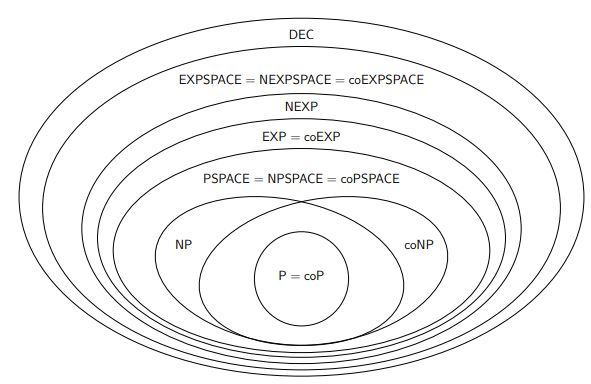
\includegraphics[width=0.7\textwidth]{images/gerarchia-classi-linguaggi-decidibili.JPG}
    %\captionof{figure}{}
\end{minipage}
\end{Thm}

\section{Classe L}
\begin{Definition}{Classi $L$ e $NL$}{}
Definiamo la classe dei linguaggi decidibili in spazio logaritmico come:
\begin{equation*}
    L = DSPACE(\log n)    
\end{equation*}
Analogamente, definiamo la classe dei linguaggi decidibili non-deterministicamente in spazio logaritmico come:
\begin{equation*}
    NL = NSPACE(\log n)    
\end{equation*}
\end{Definition}

\begin{Corollario}{Rapporto tra $L$ e $P$}{}
Date le classi $L$, $NL$ e $P$, si ha che:
\begin{equation*}
    L\subseteq NL\subseteq P    
\end{equation*}
(segue dal Teorema \ref{thm:spazio-limitante-tempo}).
\end{Corollario}

\begin{Osservation}{$NL = L$?}{}
Tramite il Teorema di Savitch, abbiamo che:
\begin{equation*}
    NL = NSPACE(\log n)\subseteq DSPACE(\log2 n)
\end{equation*}
ma non sappiamo se $NL = L$. Spesso si dice che $NL\subseteq L^2$.

A differenza delle classi $NP$ e $NEXP$, nel caso della classe $NL$ la definizione alternativa tramite verificatore ha bisogno di un piccolo cambiamento al fine di poter rispettare i vincoli di spazio:
\begin{itemize}
    \item Vincolando il certificato ad una lunghezza logaritmica otteniamo un sottoinsieme troppo ristretto di problemi in quanto il certificato risulta troppo piccolo, dunque l’insieme dei problemi verificabili in spazio logaritmi con un certificato logaritmico non coinciderebbe con $NL$.
    \item Mantenendo il certificato di lunghezza polinomiale, esso può essere utilizzato come memoria aggiuntiva: potremmo leggere più volte la stessa informazione evitando di doverla memorizzare nel work tape, risparmiando una notevole quantità di spazio.
\end{itemize}
In altre parole, nel primo caso otteniamo dei verificatori troppo deboli, mentre nel secondo sono troppo potenti. Per ottenere una via di mezzo tra le due cose, possiamo tuttavia imporre che il certificato sia read-once: il verificatore possiede un nastro aggiuntivo contenente il certificato le cui celle possono essere lette una sola volta (dunque la testina non può spostarsi a sinistra). In tal modo, preserviamo la possibilità che il certificato sia di lunghezza polinomiale ed impediamo che esso possa essere utilizzato come memoria aggiuntiva.
\end{Osservation}

\begin{Thm}{Classe $NL$ (definizione alternativa)}{}
Data la classe $NL$, si ha che:
\begin{equation*}
    NL = \{A\in DEC | \exists V\textit{ verif. con cert. read-once in spazio logaritmico per }A\}    
\end{equation*}
In altre parole, possiamo definire $NL$ anche come la classe dei linguaggi verificabili in spazio logaritmico con un certificato read-once.
\begin{demonstration}
Analizziamo la prima implicazione. Dato $A\in NL$, sia $N$ la $NTM$ tale che $A = L(N)$. Durante la sua computazione, $N$ effettuerà una serie di scelte, creando così il suo albero di computazione. Sia $V$ la TM definita come: 

$V =$ "Data la stringa $\langle w, c\rangle$ in input:
\begin{enumerate}
    \item Interpreta $c$ come una serie di scelte da effettuare
    \item Simula $N$ su input $w$ eseguendo le scelte dettate da $c$ leggendole in sequenza
    \item Se la simulazione accetta, $V$ accetta. Altrimenti, rifiuta"
\end{enumerate}
Per costruzione stessa di $V$, si ha che:
\begin{align*}
w\in L = L(N) \iff\textit{ Esiste un ramo di }N\textit{ che accetta }w\iff\\
\exists c\in \Sigma^*,\langle w, c\rangle\in L(V)
\end{align*}
dunque $V$ risulta essere un verificatore con certificato read-once di $L = L(N)$.

Inoltre, poiché $A = L(N)\in NL$, lo spazio massimo utilizzato da ogni ramo dell’albero di computazione risulta essere $O(\log n)$ e poiché la lettura del certificato non influenza lo spazio, concludiamo che $V$ sia un verificatore in spazio logaritmico.

Per la seconda implicazione. Dato un linguaggio $A$, supponiamo che esista un verificatore con certificato read-once $V$ che verifica $A$ in spazio logaritmico, implicando che:
\begin{equation*}
    \exists k\in N | V\textit{ verifica }L\textit{ in spazio }O(\log n)    
\end{equation*}
Sia $N$ la NTM definita come:

$N =$ "Data la stringa $\langle w\rangle$ in input:
\begin{enumerate}
    \item Scegli non deterministicamente una stringa $c$
    \item Simula $V$ su input $\langle w, c\rangle$
    \item Se la simulazione accetta, $B$ accetta. Altrimenti, rifiuta"
\end{enumerate}
Per costruzione stessa di $N$, si ha che
\begin{align*}
    w\in A\iff \exists c\in \Sigma^*,\langle w, c\rangle\in V\iff\\
\textit{Esiste un ramo di }N\textit{ che accetta }w\iff x\in A    
\end{align*}
implicando che $A = L(N)$.

Notiamo che le prime due operazioni di $N$ possano essere svolte in contemporanea, generando il prossimo simbolo della stringa ad ogni passo di computazione. Inoltre, poiché $V$ è un verificatore read-once in spazio logaritmico, non è sufficiente mantenere memorizzate le celle precedentemente generate. Dunque, è sufficiente memorizzare un solo simbolo per volta, richiedendo spazio $O(\log n)$. 

Dunque, concludiamo che $A = L(N)\in NL$.
\end{demonstration}
\end{Thm}

\begin{Definition}{Classe $coL$}{}
Definiamo la classe dei linguaggi $coL$ come:
\begin{equation*}
    coL = \{A\in DEC | \overline{A}\in L\}
\end{equation*}
\end{Definition}
\begin{Thm}{Chiusura del complemento di $L$}{}
Date le classi $L$ e $coL$, si ha che: 
\begin{equation*}
    L = coL
\end{equation*}
In altre parole, la classe $L$ è chiusa nel complemento (dimostrazione analoga al Teorema \ref{thm:chiusura-comp-P}).
\end{Thm}

\section{Riduzione in spazio logaritmico}
\begin{Definition}{Riducibilità in spazio logaritmico}{}
Dati due linguaggi $A$ e $B$, diciamo che $A$ è riducibile in spazio logaritmico a $B$ tramite mappatura, indicato come $A\leq^L_m B$, se esiste una funzione calcolabile $f : \Sigma^*\to \Sigma^*$, detta riduzione in spazio logaritmico da $A$ a $B$, tale che:
\begin{equation*}
    w\in A\iff f(w)\in B    
\end{equation*}
e $f$ è calcolabile in spazio logaritmico.
\end{Definition}

\begin{Thm}{Decidibilità logaritmica tramite riduzione}{}\label{thm:decidibilità-logica-riduzione}
Dati due linguaggi $A$ e $B$ tali che $A\leq^L_m B$, si ha che:
\begin{equation*}
    B\in L\implies A\in L    
\end{equation*}
\begin{demonstration}
Dato $B\in DEC$, sia $D_B$ il decisore tale che $L(D_B) = B$. Sia $D_A$ la TM definita come:

$D_A =$ "Data la stringa $w$ in input:
\begin{enumerate}
    \item Calcola $f(w)$
    \item Esegui il programma di $D_B$ con input $f(w)$.
    \item Se l’esecuzione accetta, $D$ accetta. Altrimenti, $D$ rifiuta"
\end{enumerate}
Per costruzione stessa di $D_A$, si ha che:
\begin{equation*}
    w\in L(D_A)\iff f(w)\in L(D_B) = B\iff w\in A    
\end{equation*}
implicando che $L(D_A) = A$.

Tuttavia, notiamo che, poiché $f(w)$ potrebbe richiedere spazio $O(\log n)$, è necessario eseguire le prime due operazioni in contemporanea, calcolando il prossimo simbolo di $f(w)$ ad ogni passo di computazione di $D_B$. Inoltre, poiché $D_B$ computa in spazio logaritmico, concludiamo che $A = L(D_A)\in L$.
\end{demonstration}
\end{Thm}

\begin{Thm}{Verificabilità logaritmica tramite riduzione}{}
Dati due linguaggi $A$ e $B$ tali che $A\leq^L_m B$, si ha che:
\begin{equation*}
    B\in NL\implies A\in NL    
\end{equation*}
(dimostrazione analoga al Teorema \ref{thm:decidibilità-logica-riduzione}).
\end{Thm}

\begin{Thm}{Riducibilità logaritmica transitiva}{}
Dati tre linguaggi $A, B, C\subseteq\Sigma^*$, si ha che:
\begin{equation*}
    A\leq^L_m B, B\leq^L_m C\implies A\leq^L_m C    
\end{equation*}
In altre parole, la relazione $\leq^L_m$ è transitiva.
\begin{demonstration}
Siano $f, g : \Sigma^*\to \Sigma^*$ le due funzioni calcolabili polinomialmente per cui rispettivamente si ha che $A\leq^L_m B$ e $B\leq^L_m C$.

Sia quindi $H$ la TM definita come:

$H =$ "Data la stringa $w$ in input:
\begin{enumerate}
    \item Calcola $f(w)$. Sia $k$ l’output di tale calcolo.
    \item Calcola $g(k)$ e restituisci l’output"
\end{enumerate}
Risulta evidente che $H$ sia la TM che calcola la funzione $g\circ f$ e che:
\begin{equation*}
    w\in A\iff f(w)\in B\iff g(f(w)) = (g\circ f)(w)\in C
\end{equation*}
Eseguendo contemporaneamente le due operazioni, ossia il prossimo simbolo di $f(w)$ assieme al prossimo simbolo di $g(k)$, è sufficiente utilizzare $2O(\log n)$ spazio, concludendo che $A\leq^L_m C$.
\end{demonstration}    
\end{Thm}

\begin{Thm}{Riducibilità logaritmica complementare}{}
Dati due linguaggi $A$ e $B$, si ha che:
\begin{equation*}
    A\leq^L_m B\iff \overline{A}\leq^L_m \overline{B}
\end{equation*}
(dimostrazione analoga al Teorema della riducibilità complementare).
\end{Thm}

\section{Classe NL-Complete}
\begin{Definition}{Classe NL-Complete}{}
Definiamo la classe dei linguaggi $NL-Completi$ come:
\begin{equation*}
    NL-Complete = \{L\in DEC | L\textit{ è }NL-Completo\}
\end{equation*}
dove un linguaggio $B$ è detto $NL-Completo$ se:
\begin{itemize}
    \item $B\in NL$
    \item $\forall A\in NL$ $A\leq^L_m B$
\end{itemize}
\end{Definition}

\begin{Thm}{NL-Completezza di $PATH$}{}
\textit{Dato il linguaggio $PATH$, si ha che $PATH\in NL-Complete$.}
\begin{demonstration}
Sia $N$ la NTM definita come:

$N =$ "Data la stringa $\langle G, s, t\rangle$ in input, dove $G = (V, E)$ è un grafo:
\begin{enumerate}
    \item Se $s = t$, accetta
    \item Calcola $|V| = m$
    \item Inizializza $currNode = s$ su un nastro secondario
    \item Ripeti le seguenti istruzioni per $i = 1, ..., m$
    \begin{enumerate}
        \item Seleziona non deterministicamente un nodo $u\in V$
        \item Se $(currNode, u)\notin E$, rifiuta
        \item Se $u = t$ accetta, altrimenti poni $currNode = u$.
    \end{enumerate}
    \item Rifiuta"
\end{enumerate}
Per costruzione stessa di $N$, si ha che:
\begin{equation*}
\langle G, s, t\rangle\in L(N)\iff\textit{ Esiste cammino }s\to t\textit{ in }G\iff \langle G, s, t\rangle \in PATH
\end{equation*}
implicando che $L(N) = PATH$.

Inoltre, poiché i cammini vengono letti nodo per nodo senza tenere traccia dei precedenti, lo spazio richiesto risulta essere $O(\log n)$, concludendo che $PATH = L(N)\in NL$.

Sia quindi $A \in NL$ e sia $N'$ una NTM tale che $A = L(N)$ in spazio $O(\log n)$.
Sia inoltre $f : \Sigma^*\to \Sigma^*$ la funzione calcolata dalla seguente TM $F$ definita come:

$F =$ "Data la stringa $w$ in input:
\begin{enumerate}
    \item Costruisci il grafo $G_{N,w}$ delle configurazioni della computazione di $N$ su input $w$ come nella dimostrazione del Teorema \ref{thm:path-decidible-log2n}
    \item Restituisci in output la stringa $\langle G_{N,w}, c_{start}, c_{accept}\rangle$
\end{enumerate}
Notiamo che:
\begin{align*}
w \in L(N')\iff\textit{ Esiste cammino }c_{start}\to c_{accept}\textit{ in }G_{N,w}\iff\\ f(w) = \langle G_{N,w}, c_{start}, c_{accept}\rangle\in PATH
\end{align*}
Inoltre, poiché la computazione contemporanea di $f(w)$ assieme a $\langle G_{N,w}, c_{start}, c_{accept}\rangle \in
PATH$ richiede spazio $O(\log n)$, concludiamo che $A\leq^L_m PATH$.
\end{demonstration}
\end{Thm}

\subsection{Teorema di Immerman-Szelepcsényi} 
\begin{Lemma}{Uguaglianza tra NL e coNL}{}
Dato un linguaggio $B\in NL-Complete$, si ha che:
\begin{equation*}
    B\in coNL \iff NL = coNL
\end{equation*}
(dimostrazione analoga al Teorema \ref{thm:uguaglianza-np-conp}).
\end{Lemma}

\begin{Thm}{Teorema di Immerman-Szelepcsényi}{}
Date le classi NL e coNL, si ha che:
\begin{equation*}
    NL = coNL    
\end{equation*}
In altre parole, la classe NL è chiusa nel complemento.

\begin{demonstration}
Poiché $PATH\in NL-Complete$, tramite il lemma precedente abbiamo che:
\begin{equation*}
    \overline{PATH}\in NL\iff PATH\in coNL\iff NL = coNL    
\end{equation*}
Vogliamo quindi dimostrare che $\overline{PATH}$ sia in NL. L’idea dietro la seguente dimostrazione risiede nella possibilità di abusare della lunghezza polinomiale del certificato: non possiamo leggere più volte le stesse celle, ma possiamo inserire nel certificato un numero adeguato di copie delle celle precedenti.

Sia $m = |V(G)|$ e siano $R_0,...,R_m$ gli insiemi dei vertici raggiungibili da $s$ con massimo $i\in [0, m-1]$ passi:
\begin{equation*}
    R_i = \{v\in V(G) | s\to v\textit{ con massimo }i\textit{ archi}\}
\end{equation*}
Assumiamo inoltre che i vertici di $G$ siano identificati da un numero.

Per ogni vertice $v\in V (G)$, verificare che $v\in R_i$ risulta molto facile: è sufficiente un certificato $\langle v_0,...,v_k\rangle$ che descriva il cammino, affinché il verificatore possa svolgere la seguente procedura:

\texttt{certify\_v\_in\_Ri} $(\langle v0, . . . , vk\rangle, i, v)$:
\begin{enumerate}
    \item Inizializza un contatore $h = 0$
    \item Verifica se $v_0 = s$. Se vero, incrementa $h$, altrimenti la procedura rifiuta.
    \item Verificare che per ogni $0 < j < k$ è vero che $(v_{j-1}, v_j)\in E(G)$. Se vero, incrementa $h$, altrimenti la procedura rifiuta.
    \item Verifica se $v_k = v$. Se vero incrementa $h$ (a questo punto avremo che $h = k$), altrimenti la procedura rifiuta.
    \item Verifica se $h\leq i$. Se vero, la procedura accetta, altrimenti rifiuta.
\end{enumerate}
Tramite tale ordine delle operazioni, la lettura del certificato risulta essere read-once. Inoltre, poiché i vertici di $G$ sono identificati da un numero, la lunghezza
massima di tale certificato risulta essere $O(m\log n)$.

La procedura riportata sopra, tuttavia, ci permette solo di certificare che $v\in R_i$, ma non che $v\notin R_i$. Tale operazione risulta difatti più complessa, la questione risulta più complessa, ma può essere strutturata con certificati ricorsivi.

Supponiamo di sapere che $|R_i| = \ell_i$ e di voler verificare che $v\notin R_i$. Consideriamo il
sotto-certificato $\langle c_{u_1},..., c_{u_{\ell_i}}\rangle$, dove $c_{u_k}$ è a sua volta un sotto-certificato che verifica se $u_k\in R_i$. Inoltre, visto che i vertici di $G$ sono identificati da un numero, affinché ogni sotto-certificato sia diverso è sufficiente verificare che $u_1 < ... u_{\ell_i}$. Definiamo quindi la seguente procedura:

\texttt{certify\_v\_not\_in\_Ri\_with\_|Ri|} $(\langle c_{u_1},..., c_{u_{\ell_i}}\rangle, i, v, \ell_i)$:
\begin{enumerate}
    \item Inizializza $w = 0$ e $k = 1$.
    \item Ripeti fino a fine certificato:
    \begin{enumerate}
        \item Verifica se $u_k\in R_i$ tramite la procedura \texttt{certify\_v\_in\_Ri} $(c_{u_k}, i, u_k)$. Se la procedura rifiuta, anche questa procedura rifiuta.
        \item Se $w\neq 0$, verifica se $w < u_k$. Se vero, poni $w = u_k$ e incrementa $k$, altrimenti rifiuta.
        \item Verifica $u_k\neq v$. Se falso, rifiuta.
    \end{enumerate}
    \item Verifica se $k = \ell_i$. Se vero accetta, altrimenti rifiuta.
\end{enumerate}
Tramite tale ordine delle operazioni, anche questo certificato risulta essere read-once. Inoltre, poiché per ogni $i$ abbiamo che $|R_i|\leq m$, il certificato contiene massimo $m$ sotto-certificati, i quali sappiamo avere lunghezza $O(m\log n)$. Per tanto, questo certificato ha lunghezza $O(m^2\log n)$.

Supponiamo invece di sapere che $|R_{i-1}| = \ell_{i-1}$ e di voler verificare che $v\notin R_i$. Similmente al caso precedente, consideriamo il sotto-certificato $\langle c_{u_1},...,c_{u_{\ell_{i-1}}}\rangle$, dove $c_{u_k}$ questa volta è un sotto-certificato che verifica se $u_k\in R_{i-1}$. La procedura risulta essere analoga alla precedente, ma con una differenza fondamentale: verifichiamo che nessuno dei vertici in $R_{i-1}$ sia un vertice adiacente a $v$.

\texttt{certify\_v\_not\_in\_Ri\_with\_|Ri-1|} $(\langle c_{u_1},..., c_{u_{\ell_{i-1}}}\rangle, i, v, \ell_{i-1})$:
\begin{enumerate}
    \item Inizializza $w = 0$ e $k = 1$.
    \item Ripeti fino a fine certificato:
    \begin{enumerate}
        \item Verifica se $u_k\in R_i$ tramite la procedura \texttt{certify\_v\_in\_Ri} $(c_{u_k}, i-1, u_k)$.
        Se la procedura rifiuta, anche questa procedura rifiuta.
        \item Se $w\neq 0$, verifica se $w < u_k$. Se vero, poni $w = u_k$ e incrementa $k$, altrimenti rifiuta.
        \item Verifica se $w\neq v$ e che $w\neq u$ per ogni vertice adiacente a $v$. Se falso, rifiuta.
    \end{enumerate}
    \item Verifica se $k = \ell_{i-1}$. Se vero accetta, altrimenti rifiuta.
\end{enumerate}
Ovviamente, anche questo certificato risulta essere read-once e la sua lunghezza è $O(m^2\log n)$.

A questo punto, è necessario definire l’ultimo step: sapendo che $|R_{i-1}| = \ell_{i-1}$, vogliamo verificare che $|R_i| = \ell_i$. Consideriamo il sotto-certificato 
$\langle c_{v_0},...,c_{v_{m-1}}\rangle$. Per ogni vertice $v$ di $G$ abbiamo solo due opzioni: il vertice appartiene a $R_i$, dunque possiamo verificare ciò tramite un certificato da dare alla prima procedura, oppure esso non appartiene a $R_i$, dunque sapendo $|R_{i-1}|$ possiamo verificare ciò tramite un certificato da dare alla terza procedura.

\texttt{certify\_|Ri-1|\_with\_|Ri-1|} $(\langle c_{v_0},...,c_{v_{m-1}}\rangle, i, \ell_i, \ell_{i-1})$:
\begin{enumerate}
    \item Inizializza un contatore $h = 0$.
    \item Ripeti per $k = 0, . . . , m-1$:
    \begin{enumerate}
        \item Verifica se $v_k\in R_i$ tramite la procedura \texttt{certify\_v\_in\_Ri} $(c_{v_k}, i, v_k)$. Se la procedura accetta, incrementa $h$.
        \item Altrimenti, verifica se $v_k\notin R_i$ tramite la procedura \texttt{certify\_v\_not\_in\_Ri\_with\_|Ri-1|}$(c_{v_k}, i, v_k, \ell_{i-1})$. Se la procedura rifiuta, anche questa procedura rifiuta.
        \item Se $h = \ell_i$ allora accetta, altrimenti rifiuta.
    \end{enumerate}
\end{enumerate}
Tale procedura dunque non fa altro che calcolare la cardinalità di $R_i$, per poi verificare se essa sia uguale al valore $\ell_i$ dato. Intuitivamente, notiamo che il certificato sia composto da $m$ altri sotto-certificati ognuno di lunghezza $O(m^2\log n)$. Per tanto, questo certificato risulta avere lunghezza $O(m^3\log n)$.

Una volta definite tutte le procedure necessarie, definiamo la seguente TM $V$:

$V =$ "Data la stringa $\langle \langle G, s, t\rangle, c\rangle$ in input:
\begin{enumerate}
    \item Interpreta $c = \langle \ell_0,...,\ell_{m-1}, c_0,...,c_{m-1}, c_t\rangle$
    \item Ripeti per $i = 0, . . . , m-1$:
    \begin{enumerate}
        \item Esegui la procedura \texttt{certify\_|Ri-1|\_with\_|Ri-1|}$(c_i, i, \ell_i, \ell_{i-1})$. Se la procedura rifiuta, anche questa procedura rifiuta.
    \end{enumerate}
    \item Esegui la procedura \texttt{certify\_v\_not\_in\_Ri\_with\_|Rm|}$(c_t, m, t, \ell_m)$. Se la procedura accetta, anche questa procedura accetta, altrimenti rifiuta.
\end{enumerate}
In altre parole, la TM $V$ utilizza i valori $\ell_0,...,\ell_{m-1}$ e i sotto-certificati $c_0,...,c_{m-1}$ per arrivare a certificare che $|R_m| = \ell_m$, per poi utilizzare il sotto-certificato $c_t$ per determinare se $t\in R_m$, concludendo quindi che $V$ sia un verificatore per $PATH$.

Poiché ognuna delle procedure risulta essere read-once e il certificato finale è composto da $m$ interi ognuno necessitante $\log n$ bit, $m + 1$ certificati ognuno necessitante $O(m^3\log n)$ bit e poiché $m$ è in $O(n)$, concludiamo che il costo spaziale del verificatore $V$ sia:
\begin{equation*}
    O(m\log n+(m + 1)(m^3\log n)) = O(n^4\log n)
\end{equation*}
e dunque che $PATH\in NL$.
\end{demonstration}
\end{Thm}